\chapter{METODE PENELITIAN}

Metode pada penelitian ini terdiri dari beberapa tahapan proses seperti yang terlihat pada Gambar 3.1.
\begin{afigure}
    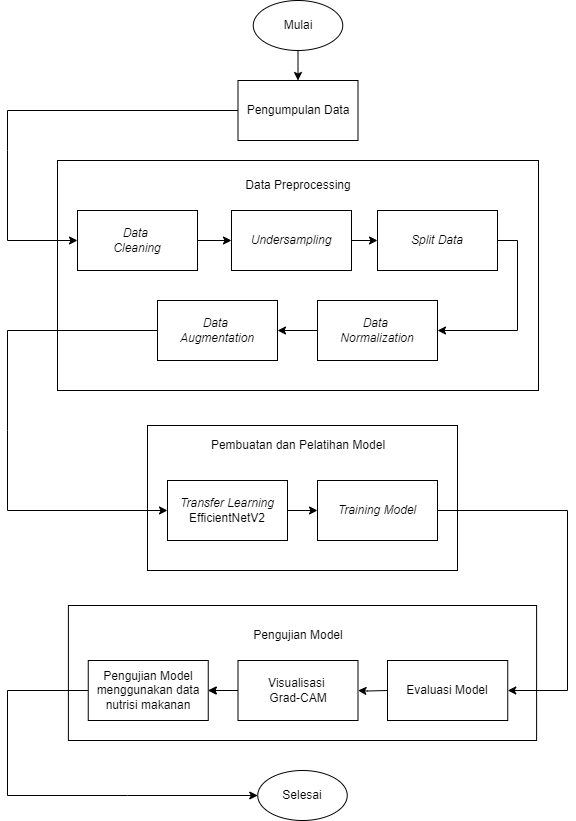
\includegraphics[height=0.74\textheight, width=0.9\textwidth, center]{images/flowchart.png}
    \caption{Flowchart Tahapan Metode Penelitian}
    \label{fig:flowchart-metode}
\end{afigure}

Tahapan awal pada penelitian ini adalah pengumpulan data citra makanan dari internet. Pada penelitian ini, data citra makanan diambil dari \textit{google images} menggunakan teknik \textit{scraping}. Tools yang digunakan dalam penelitian ini yaitu Google Image Scraper. Total dataset citra yang berhasil dikumpulkan sebanyak 5000 citra yang terbagi dalam 10 kelas (ayam bakar, bakso, gado-gado, gudeg, nasi goreng, pempek, rawon, rendang, sate, dan soto) dimana setiap kelas memiliki total 500 citra makanan. Setelah data terkumpul, langkah selanjutnya adalah \textit{preprocessing data} yang melibatkan beberapa tahapan, yaitu pembersihan data (\textit{data cleaning}) untuk memastikan data bebas dari kesalahan dan inkonsistensi, undersampling untuk menangani ketidakseimbangan data, pembagian data (\textit{split data}) menjadi set pelatihan dan set pengujian, augmentasi data (\textit{data augmentation}) untuk memperluas jumlah data pelatihan dengan membuat variasi dari data yang sudah ada, dan normalisasi data (\textit{data normalization}) untuk membuat data menjadi lebih banyak variasi.

Setelah tahap \textit{preprocessing} selesai, proses dilanjutkan dengan pembuatan dan pelatihan model. Pada penelitian ini, pelatihan model akan menggunakan 2 GPU yang berbeda, yang pertama yaitu menggunakan Google Colab dengan GPU T4, kemudian yang kedua menggunakan mesin DGX A100 dari Universitas Gunadarma. Tahapan ini melibatkan \textit{transfer learning} menggunakan EfficientNetV2, sebuah arsitektur jaringan saraf yang telah dilatih sebelumnya pada sejumlah besar data. Model yang dihasilkan dari \textit{transfer learning} kemudian dilatih lebih lanjut menggunakan data yang telah melalui tahap \textit{preprocessing}.

Tahap berikutnya adalah pengujian model. Langkah ini mencakup evaluasi model untuk mengukur kinerjanya, visualisasi Grad-CAM untuk memahami bagaimana model mengambil keputusan dengan memvisualisasikan bagian dari gambar yang diperhatikan oleh model, dan pengujian model akhir menggunakan data nutrisi makanan untuk memastikan model berfungsi dengan baik dalam konteks yang diinginkan.

\section{Pengumpulan Data}
Pada tahapan ini, dataset dikumpulkan melalui internet. Pada penelitian ini, data citra makanan diambil dari \textit{google images} menggunakan teknik \textit{scraping}. Tools yang digunakan dalam penelitian ini yaitu \textit{google image scraper}. Total dataset citra yang berhasil dikumpulkan sebanyak 2000 citra yang terbagi dalam 10 kelas (ayam bakar, bakso, gado-gado, gudeg, nasi goreng, pempek, rawon, rendang, sate, dan soto) dimana setiap kelas memiliki total 200 citra makanan.

Berikut ini merupakan langkah-langkah yang dilakukan untuk mengumpulkan data citra makanan menggunakan teknik \textit{scraping} menggunakan \textit{Google Image Scraper}:
\begin{enumerate}
    \item Pastikan komputer sudah terinstall git. lalu lakukan clone menggunakan \textit{command prompt} 'git clone https://github.com/ohyicong/Google-Image-Scraper'
    \item Lalu lakukan instalasi \textit{dependency} menggunakan \textit{command prompt} 'pip install -r requirements.txt'
    \item Buka file 'main.py', lalu ganti kode pada variabel 'search\_keys' sesuai kata kunci yang diinginkan. Pada penelitian ini, kata kunci yang digunakan yaitu ayam bakar, bakso, gado gado, gudeg, nasi goreng, pempek, rawon, rendang, sate, dan soto.
    \item Kemudian ganti juga kode nilai pada variabel 'number\_of\_images' sesuai dengan jumlah citra yang diinginkan. Pada penelitian ini, citra yang diinginkan berjumlah 500 citra. Pastikan simpan file main.py setelah dilakukan pengubahan kode.
    \begin{afigure}
        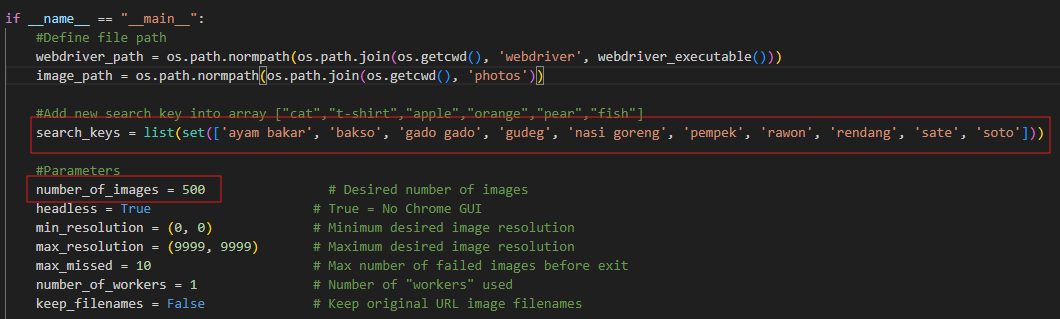
\includegraphics[width=0.9\textwidth, center]{images/kode1.png}
        \caption{Tampilan kode main.py}
        \label{fig:main.py}
    \end{afigure}
    \item Buka \textit{command prompt}, lalu jalankan program menggunakan 'python main.py'. Proses \textit{scraping} akan berjalan dalam waktu yang cukup lama.
    \item Setelah proses \textit{scraping} selesai, citra akan tersimpan pada folder 'photos'. Hasilnya dapat dilihat pada Gambar 3.3
    \begin{afigure}
        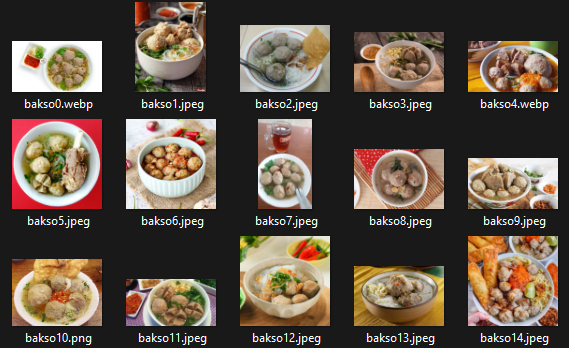
\includegraphics[width=0.9\textwidth, center]{images/kode2.png}
        \caption{Hasil scraping menggunakan Google Image Scraper}
        \label{fig:scraping}
    \end{afigure}
\end{enumerate}

\section{\textit{Data Preprocessing}}
Setelah dilakukan pengumpulan dataset, selanjutnya yaitu dilakukan \textit{Data Preprocessing} pada data citra. Ada beberapa tahapan dalam \textit{Data Preprocessing}, yaitu \textit{Data Cleaning}, \textit{Undersampling}, \textit{Split Data}, \textit{Data Augmentation}, dan \textit{Data Normalization}. Dalam proses ini dibutuhkan beberapa \textit{package} Python yang harus diinstalasi dan dipanggil saat program dijalankan di Jupyter Notebooks, yaitu:

\begin{lstlisting}[style=customc]
import splitfolders
import os
from keras.preprocessing.image import ImageDataGenerator
import matplotlib.pyplot as plt
import numpy as np
import cv2
\end{lstlisting}

\begin{itemize}
    \item \textit{Library} 'splitfolders' digunakan untuk membagi dataset menjadi data latih dan data pengujian.
    \item \textit{Library} 'os' digunakan untuk membantu inisialisasi variabel data latih dan data pengujian berdasarkan nama folder.
    \item 'from keras.preprocessing.image import ImageDataGenerator' digunakan untuk mengambil fungsi ImageDataGenerator dari \textit{library} Keras. ImageDataGenerator digunakan untuk melakukan \textit{Image Normalization} dan \textit{Image Augmentation}
    \item \textit{Library} 'matplotlib' disingkat 'plt' digunakan untuk visualisasi
    \item \textit{Library} 'numpy' disingkat 'np' digunakan untuk operasi matematika dan manipulasi array.
    \item \textit{Library} 'cv2' digunakan untuk manipulasi data berbentuk citra.
\end{itemize}

\subsection{\textit{Data Cleaning}}
Pada tahap \textit{Data Cleaning}, data citra yang berhasil dikumpulkan dilakukan pembersihan. Proses ini dilakukan untuk memastikan data bebas dari kesalahan dan inkonsistensi. Hal ini dilakukan karena data citra yang didapatkan dari \textit{scraping} banyak yang \textit{duplicate} dan banyak citra yang tidak sesuai dengan makanan yang dimaksud.
\begin{afigure}
    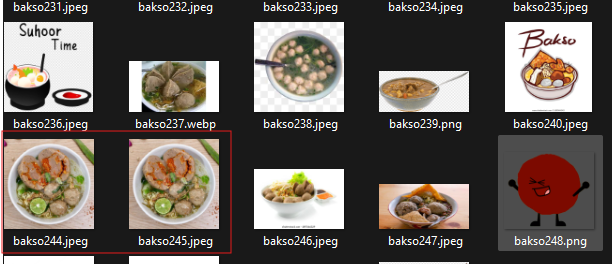
\includegraphics[width=0.9\textwidth, center]{images/duplicate.png}
    \caption{Contoh Citra Duplicate}
    \label{fig:duplicate}
\end{afigure}

Pada Gambar 3.4 terlihat file citra dengan nama 'bakso244.jpeg' dengan 'bakso245.jpeg' merupakan citra yang sama atau disebut \textit{duplicate}. Hal ini terjadi di banyak kelas, tidak hanya di kelas 'bakso'. Pada Gambar 3.5 terihat beberapa file citra banyak yang tidak sesuai dengan kelasnya, seperti gambar kartun ataupun poster promosi.

\begin{afigure}
    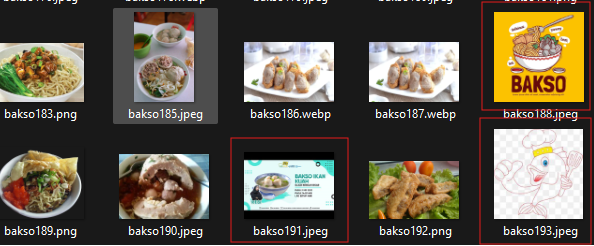
\includegraphics[width=0.9\textwidth, center]{images/inconsistent-image.png}
    \caption{Contoh Citra yang tidak sesuai}
    \label{fig:inconsistent}
\end{afigure}

Pada penelitian ini, tahap \textit{Data Cleaning} dilakukan secara manual. Langkah pertama dalam proses \textit{Data Cleaning} adalah pemeriksaan awal citra makanan. Setiap citra diperiksa untuk memastikan bahwa resolusi dan kualitasnya memadai untuk analisis lebih lanjut. Citra yang buram, terlalu gelap, atau terlalu terang dihapus dari dataset. Selain itu, citra yang tidak relevan atau tidak sesuai dengan kategori makanan yang diteliti juga dieliminasi.

Langkah kedua adalah deteksi anomali. Citra yang memiliki \textit{noise} atau artefak yang tidak diinginkan diidentifikasi dan dieliminasi. Misalnya, citra yang memiliki bayangan berlebihan atau adanya objek asing yang mengganggu akan dieliminasi.

Tahap terakhir dalam proses \textit{Data Cleaning} adalah validasi dan verifikasi. Setelah semua langkah di atas dilakukan, citra makanan yang telah dibersihkan diverifikasi kembali untuk memastikan bahwa tidak ada kesalahan yang terlewatkan. Citra yang lolos tahap ini kemudian siap digunakan untuk analisis lebih lanjut.

\subsection{\textit{Undersampling}}
Pada tahapan ini, data citra yang telah dibersihkan melalui tahap \textit{data cleaning} kemudian dilakukan proses \textit{undersampling}. \textit{Undersampling} dilakukan untuk menangani ketidakseimbangan data yang ada dalam dataset. Ketidakseimbangan data terjadi ketika jumlah citra dalam satu kelas makanan jauh lebih banyak dibandingkan dengan kelas lainnya. Langkah-langkah dalam proses \textit{undersampling} pada data citra ini meliputi:
\begin{enumerate}
    \item \textbf{Identifikasi Ketidakseimbangan Data} 
    \item[] Langkah pertama adalah mengidentifikasi ketidakseimbangan dalam dataset. Hal ini dilakukan dengan menghitung jumlah citra dalam setiap kelas makanan dan menentukan kelas mana yang memiliki jumlah sampel yang jauh lebih banyak dibandingkan kelas lainnya.
    \item \textbf{Pemilihan Sampel untuk \textit{Undersampling}} 
    \item[] Setelah mengidentifikasi kelas mayoritas, langkah selanjutnya adalah memilih sejumlah sampel dari kelas tersebut untuk dihapus. Pemilihan sampel ini dapat dilakukan secara acak atau menggunakan metode tertentu yang mempertimbangkan distribusi data untuk menjaga keragaman sampel yang tersisa.
    \item \textbf{Penghapusan Sampel Kelas Mayoritas} 
    \item[] Hapus sampel yang telah dipilih dari kelas mayoritas. Penghapusan ini dilakukan dengan hati-hati untuk memastikan bahwa sampel yang tersisa masih representatif dan mencakup berbagai variasi dalam kelas tersebut.
    \item \textbf{Validasi Dataset Baru} 
    \item[] Setelah melakukan \textit{undersampling}, penting untuk memvalidasi dataset baru. Proses validasi ini memastikan bahwa data yang tersisa masih representatif dan tidak mengandung bias yang dapat mempengaruhi hasil analisis. Validasi juga memastikan bahwa tidak ada informasi penting yang hilang dari kelas mayoritas.
\end{enumerate}

\subsection{Split Data}
Setelah melewati tahapan \textit{Undersampling}, kemudian dilakukan proses \textit{Split Data}. \textit{Split Data} merupakan proses untuk membagi data menjadi data latih dan data uji. Pada penelitian ini, proses \textit{Split Data} menggunakan \textit{library} 'split-folders' dengan rasio 80\% data latih dan 20\% data uji. Untuk melakukan \textit{Split Data}, digunakan perintah sebagai berikut:

\begin{lstlisting}[style=customc]
!pip install split-folders
import splitfolders
splitfolders.ratio('/content/dataset', 
output="split_images", seed=1337, ratio=(.8,.2))
\end{lstlisting}

Keterangan sintaks:
\begin{itemize}
    \item '!pip install split-folders' digunakan untuk instalasi 'split-folders'
    \item 'import splitfolders' digunakan untuk memanggil fungsi splitfolders agar dapat digunakan.
    \item 'splitfolders.ratio' merupakan fungsi dari \textit{library} 'splitfolders' untuk \textit{Split Data}.
    \item '/content/dataset' merupakan folder dataset.
    \item 'output="split\_images" merupakan folder output.
    \item 'seed=1337' digunakan agar pembagian dataset tetap sama dan tidak random setiap menjalankan perintah ini.
    \item 'ratio=(.8,.2)' merupakan rasio pembagian dataset 80\% untuk data latih dan 20\% untuk data uji.
\end{itemize}

\subsection{\textit{Data Normalization}}
Tahapan selanjutnya yaitu \textit{Data Normalization}. Pada tahapan ini, data citra yang telah dibagi menjadi data latih dan data uji kemudian dilakukan proses normalisasi data. Proses \textit{data normalization} digunakan untuk menyesuaikan skala nilai piksel pada sebuah gambar sehingga rentang nilai pikselnya menjadi lebih konsisten. Tujuannya adalah untuk meningkatkan performa model \textit{machine learning} dalam mempelajari pola gambar tanpa adanya bias dari perbedaan skala nilai piksel. Pada proses \textit{image normalization} setiap nilai piksel citra dibagi dengan 255. Kemudian data citra diubah menjadi ukuran 224 x 224 x 3.

\subsection{\textit{Data Augmentation}}
Tahapan akhir pada \textit{Data Preprocessing} yaitu tahapan \textit{Data Augmentation}. \textit{Data Augmentation} digunakan untuk memperluas dataset dengan membuat variasi pada gambar-gambar yang ada dengan cara melakukan transformasi pada gambar asli. Tujuannya dapat mencegah \textit{overfitting}, mencegah adanya bias dan meningkatkan akurasi. Proses \textit{Data Normalization} dan \textit{Data Augmentation} diimplementasikan ke dalam bentuk kode seperti yang dapat dilihat pada blok program di bawah:

\begin{lstlisting}[style=customc]
batch_size = 16

train_datagen = ImageDataGenerator(
                    preprocessing_function=preprocess_input,
                    rotation_range = 40,
                    shear_range = 0.2,
                    zoom_range = 0.2,
                    horizontal_flip = True,
                    vertical_flip = True)

val_datagen = ImageDataGenerator(
                    preprocessing_function=preprocess_input)


train_dataset = train_datagen.flow_from_directory(
        train_dir,
        shuffle=False,
        target_size=(224, 224),
        batch_size=batch_size,
        class_mode='categorical')

val_dataset = val_datagen.flow_from_directory(
        val_dir,
        shuffle=False,
        target_size=(224, 224),
        batch_size=batch_size,
        class_mode='categorical')
\end{lstlisting}

Proses \textit{Data Normalization} dan \textit{Data Augmentation} dilakukan menggunakan fungsi ImageDataGenerator dari \textit{library} tensorflow. Untuk proses \textit{Data Normalization} dilakukan menggunakan sintaks 'preprocessing\_function', dan data citra diubah menjadi ukuran 224 x 224 x 3 dilakukan menggunakan sintaks 'target\_size(224, 224). Kemudian proses \textit{Data Augmentation} dilakukan hanya pada data latih dengan keterangan sebagai berikut:
\begin{enumerate}
    \item 'rotation\_range = 40' digunakan untuk melakukan rotasi pada data citra sebesar 40 derajat.
    \item 'shear\_range = 0.2' digunakan untuk menentukan intensitas shear (sudut shear dalam arah berlawanan jarum jam dalam derajat) sebagai fraksi dari lebar citra sebesar 20\%.
    \item 'zoom\_range =0.2' digunakan untuk \textit{zoom in} atau \textit{zoom out} citra secara acak hingga 20\%.
    \item 'horizontal\_flip = True' digunakan untuk membalik citra secara acak secara horizontal.
    \item 'vertical\_flip = True' digunakan untuk membalik citra secara acak secara vertical.
\end{enumerate}

\section{Pembuatan dan Pelatihan Model}
Data citra yang sudah melewati proses \textit{Data Preprocessing} kemudian dilakukan proses Pembuatan dan Pelatihan model. Pada penelitian ini, pelatihan model akan menggunakan 2 GPU yang berbeda, yang pertama yaitu menggunakan Google Colab dengan GPU T4, kemudian yang kedua menggunakan mesin DGX A100 dari Universitas Gunadarma. Pada proses ini, ada 2 tahapan yaitu tahapan \textit{Transfer Learning} menggunakan \textit{EfficientNetV2} dan \textit{Training Model}. Dalam proses ini dibutuhkan beberapa \textit{package} Python yang harus diinstalasi dan dipanggil saat program dijalankan di Jupyter Notebooks, yaitu

\begin{lstlisting}[style=customc]
from tensorflow.keras.applications import EfficientNetV2S
from keras.layers import Input
from keras import layers
from tensorflow.keras.callbacks import ModelCheckpoint
import time
\end{lstlisting}

Keterangan sintaks:
\begin{itemize}
    \item 'from tensorflow.keras.applications import EfficientNetV2S' digunakan untuk memanggil fungsi 'EfficientNetV2S' dari \textit{library} tensorflow yang akan digunakan untuk proses \textit{Transfer Learning}.
    \item 'from keras.layers import Input' digunakan untuk memanggil fungsi 'Input' dari \textit{library} keras yang akan digunakan untuk menentukan input layer pada model.
    \item 'from keras import layers' digunakan untuk memanggil fungsi 'layers' dari \textit{library} keras yang akan digunakan untuk membuat layer-layer pada model.
    \item 'from tensorflow.keras.callbacks import ModelCheckpoint' digunakan untuk memanggil fungsi 'ModelCheckPoint' dari \textit{library} tensorflow yang akan digunakan untuk membuat checkpoint model terbaik pada saat \textit{training model}.
    \item 'import time' digunakan untuk mencatat lama waktu training.
\end{itemize}

\subsection{\textit{Transfer Learning} EfficientNetV2}
Tahapan pertama pada proses \textit{Pembuatan dan Pelatihan Model} yaitu tahap \textit{Transfer Learning} menggunakan EfficientNetV2. Pada penelitian ini model pra-terlatih yang digunakan merupakan EfficientNetV2S. EfficientNetV2S merupakan model pra-terlatih dari EfficientNetV2 yang terkecil. Pada penelitian ini, proses \textit{transfer learning} dilakukan menggunakan \textit{pre-trained weights} dari dataset ImageNet. ImageNet berisi lebih dari 14 juta gambar yang diberi label dalam 1000 kategori. Ini mencakup berbagai objek dan skenario, memberikan model dasar yang kuat dengan representasi visual yang luas dan beragam. Dengan menggunakan bobot yang telah dilatih sebelumnya (\textit{pre-trained weights}), kita dapat memanfaatkan pengetahuan yang telah diperoleh oleh model tersebut tanpa perlu melatihnya dari awal. Ini tidak hanya menghemat waktu tetapi juga biaya komputasi. Proses \textit{Transfer Learning} menggunakan EfficientNetV2S diimplementasikan ke dalam bentuk kode seperti yang dapat dilihat pada blok program di bawah:

\begin{lstlisting}[style=customc]
pre_trained_model = EfficientNetV2S(weights='imagenet', 
include_top=False, input_tensor=Input(shape=(224, 224, 3)))

pre_trained_model.trainable = False

x = pre_trained_model.output
x = layers.GlobalAveragePooling2D()(x)
outputs = layers.Dense(n_classes, activation='softmax')(x)
model = tf.keras.models.Model(
pre_trained_model.input, outputs)
\end{lstlisting}

Keterangan sintaks:
\begin{itemize}
    \item 'EfficientNetV2S': Ini adalah arsitektur model yang dipilih, yaitu EfficientNet versi 2 dengan ukuran S (small).
    \item 'weights='imagenet'': Model ini menggunakan bobot yang telah dilatih sebelumnya pada dataset ImageNet.
    \item 'include\_top=False': Hanya menggunakan bagian dasar dari model (tanpa lapisan dense terakhir atau "top" layer yang biasanya digunakan untuk klasifikasi pada 1000 kelas ImageNet).
    \item 'input\_tensor=Input(shape=(224, 224, 3))': Menentukan bentuk input dari gambar yang akan diproses oleh model, yaitu gambar dengan ukuran 224x224 piksel dan 3 saluran warna (RGB).
    \item 'trainable = False': Dengan mengatur trainable menjadi False, perintah ini akan mengunci semua bobot dalam model sehingga tidak akan diperbarui selama proses pelatihan. Ini berarti bobot akan tetap sama seperti bobot awal yang dimuat dari ImageNet.
    \item 'pre\_trained\_model.output': Ini mengambil output dari lapisan terakhir model pra-terlatih (EfficientNetV2S). Output ini akan menjadi input untuk lapisan tambahan yang akan ditambahkan.
    \item 'layers.GlobalAveragePooling2D()': Ini adalah lapisan pooling yang mengurangi dimensi spasial dari fitur peta (\textit{feature map}) yang dihasilkan oleh model pra-terlatih. Global Average Pooling menghitung rata-rata dari setiap peta fitur dan mengurangi data menjadi satu vektor per peta fitur.
    \item 'layers.Dense(n\_classes, activation='softmax')': Ini adalah lapisan dense (\textit{fully connected layer}) dengan jumlah neuron sebanyak n\_classes (10 kelas). Aktivasi softmax digunakan untuk mengonversi output menjadi probabilitas kelas untuk tugas klasifikasi.
    \item 'tf.keras.models.Model(pre\_trained\_model.input, outputs)': Ini mendefinisikan model baru dengan input sama seperti input dari model pra-terlatih dan output sebagai output dari lapisan dense yang baru saja kita tambahkan. Model ini sekarang terdiri dari model pra-terlatih (yang bobotnya terkunci) dan lapisan baru yang akan dilatih.
\end{itemize}

\subsection{\textit{Training Model}}
Setelah membuat model baru menggunakan metode \textit{Transfer Learning} menggunakan EfficientNetV2S, dilakukan proses \textit{training model} atau pelatihan model. Pada penelitian ini, pelatihan model akan menggunakan 2 GPU yang berbeda, yang pertama yaitu menggunakan Google Colab dengan GPU T4, kemudian yang kedua menggunakan mesin DGX A100 dari Universitas Gunadarma. Tahap pertama yang dilakukan yaitu melakukan kompilasi model. Proses kompilasi model diimplementasikan ke dalam bentuk kode seperti yang dapat dilihat pada blok program di bawah:

\begin{lstlisting}[style=customc]
model.compile(
    optimizer=tf.keras.optimizers.Adam(learning_rate=0.001),
    loss='categorical_crossentropy',
    metrics=['accuracy']
)
\end{lstlisting}

Keterangan sintaks:
\begin{itemize}
    \item 'tf.keras.optimizers.Adam': Adam (\textit{Adaptive Moment Estimation}) adalah algoritma pengoptimalan yang sering digunakan dalam pembelajaran mendalam karena menggabungkan kelebihan dari dua algoritma optimasi lainnya, yaitu AdaGrad dan RMSProp. Adam bekerja dengan menyimpan perkiraan rata-rata momentum dari gradien serta kuadrat dari gradien.
    \item 'learning\_rate=0.001': Ini adalah parameter laju pembelajaran yang digunakan oleh optimizer. Laju pembelajaran menentukan seberapa besar pembaruan bobot yang dilakukan pada setiap iterasi pelatihan. Nilai 0.001 adalah nilai umum yang sering digunakan karena memberikan keseimbangan yang baik antara kecepatan konvergensi dan stabilitas.
    \item 'categorical\_crossentropy': Ini adalah fungsi kehilangan (\textit{loss function}) yang digunakan untuk masalah klasifikasi dengan lebih dari dua kelas (klasifikasi multi-kelas). \textit{Categorical crossentropy} mengukur perbedaan antara distribusi probabilitas yang diprediksi dan distribusi sebenarnya (\textit{ground truth}).
    \item 'accuracy': Metrik yang digunakan untuk mengevaluasi kinerja model selama pelatihan dan pengujian. Akurasi adalah metrik yang umum digunakan yang menunjukkan persentase prediksi model yang benar. Dalam konteks klasifikasi multi-kelas, akurasi mengukur seberapa sering prediksi kelas dari model sesuai dengan label kelas sebenarnya.
\end{itemize}

Tahap kedua yaitu melakukan inisialisasi \textit{checkpointer}. \textit{Checkpointer} menggunakan fungsi callback 'ModelCheckpoint' dari \textit{library} tensorflow. Pada penelitian ini, callback digunakan untuk menyimpan model selama pelatihan berdasarkan performa terbaik pada dataset validasi. Proses inisialisasi \textit{checkpointer} diimplementasikan ke dalam bentuk kode seperti yang dapat dilihat pada blok program di bawah:
\begin{lstlisting}[style=customc]
checkpointer = ModelCheckpoint(
    filepath='best_model.h5',
    monitor='val_loss',
    verbose=1,
    save_best_only=True,
    mode='min'
)
\end{lstlisting}
Keterangan sintaks:
\begin{itemize}
    \item 'best\_model.h5': Ini adalah folder di mana model terbaik akan disimpan. File dengan ekstensi .h5 menunjukkan bahwa model akan disimpan dalam format HDF5, yang merupakan format populer untuk menyimpan model Keras.
    \item 'val\_loss': Parameter ini menentukan metrik yang akan dipantau untuk menentukan apakah model yang sedang dilatih mengalami perbaikan. Dalam kasus ini, metrik yang dipantau adalah val\_loss (loss pada data validasi).
    \item 'save\_best\_only=True': Jika diatur ke True, model hanya akan disimpan jika perbaikan pada metrik yang dipantau (dalam hal ini val\_loss) ditemukan. Ini berarti model hanya akan disimpan ketika ia menunjukkan kinerja yang lebih baik dibandingkan semua iterasi sebelumnya.
    \item 'mode=min': Parameter ini menentukan apakah model yang lebih baik adalah model dengan nilai lebih rendah ('min') atau lebih tinggi ('max') dari metrik yang dipantau. Dalam kasus ini, mode 'min' berarti model dengan val\_loss terendah akan disimpan.
\end{itemize}

Setelah kompilasi dan inisialisasi \textit{checkpointer}, tahap terakhir yaitu melakukan \textit{training model} atau pelatihan model menggunakan TensorFlow. Pada penelitian ini, jumlah epoch yang dipakai yaitu 50 epoch. Proses \textit{training model} diimplementasikan ke dalam bentuk kode seperti yang dapat dilihat pada blok program di bawah:

\begin{lstlisting}[style=customc]
num_epochs = 50
start_time = time.time()

history = model.fit(train_dataset,
                epochs=num_epochs,
                validation_data=val_dataset,
                callbacks=[checkpointer]
                )

elapsed_time = time.time() - start_time
time.strftime("%H:%M:%S", time.gmtime(elapsed_time))
\end{lstlisting}

Keterangan sintaks:
\begin{itemize}
    \item 'num\_epoch's = 50: Mengatur jumlah epoch untuk pelatihan model. Satu epoch adalah satu siklus penuh melalui seluruh dataset pelatihan. Dalam kasus ini, model akan dilatih selama 50 epoch.
    \item 'start\_time = time.time()': Menyimpan waktu mulai pelatihan dalam satuan detik. Ini digunakan untuk menghitung berapa lama waktu yang dibutuhkan untuk melatih model.
    \item 'model.fit': Metode ini digunakan untuk melatih model dengan dataset pelatihan.
    \item 'train\_dataset': Dataset yang digunakan untuk melatih model.
    \item 'epochs=num\_epochs': Menentukan jumlah epoch untuk pelatihan, yaitu 50 epoch.
    \item 'validation\_data=val\_dataset': Dataset yang digunakan untuk validasi model selama pelatihan. Performansi model pada dataset ini digunakan untuk memantau \textit{overfitting}.
    \item 'callbacks=[checkpointer]': Daftar callback yang digunakan selama pelatihan. Dalam hal ini, checkpointer adalah callback ModelCheckpoint yang telah diinisialisasi sebelumnya, yang digunakan untuk menyimpan model terbaik selama pelatihan.
    \item 'elapsed\_time = time.time() - start\_time': Menghitung selisih waktu antara waktu selesai pelatihan dan waktu mulai pelatihan. Ini memberikan total waktu yang dibutuhkan untuk melatih model dalam satuan detik.
    \item 'time.strftime("\%H:\%M:\%S", time.gmtime(elapsed\_time))': Mengubah waktu yang dihitung (elapsed\_time) menjadi format yang lebih mudah dibaca (jam:menit)
\end{itemize}

\section{Pengujian Model}
Setelah dilakukan proses \textit{Data Preprocessing}, selanjutnya yaitu dilakukan Pengujian Model. Pengujian Model merupakan proses terakhir dari penelitian ini. Pada proses ini dibagi menjadi 3 tahapan, yaitu Evaluasi Model, Visualisasi Grad-CAM dan Pengujian Model menggunakan data nutrisi makanan. Dalam proses ini dibutuhkan beberapa \textit{package} Python yang harus diinstalasi dan dipanggil saat program dijalankan di Jupyter Notebooks, yaitu:
\begin{lstlisting}[style=customc]
from sklearn.metrics import accuracy_score,
classification_report, confusion_matrix,
ConfusionMatrixDisplay
\end{lstlisting}

Keterangan sintaks:
\begin{itemize}
    \item 'sklearn.metrics': merupakan kode untuk menggunakan kelas metrics dari library sklearn atau scikit-learn.
    \item 'accuracy\_score': Fungsi ini menghitung akurasi klasifikasi, yang merupakan rasio prediksi benar dibandingkan dengan total prediksi. Ini adalah metrik evaluasi yang paling dasar untuk masalah klasifikasi.
    \item 'classification\_report': Fungsi ini menghasilkan laporan yang menunjukkan metrik kinerja utama untuk masalah klasifikasi, seperti \textit{precision}, \textit{recall}, \textit{f1-score}, dan \textit{support} untuk setiap kelas.
    \item 'confusion\_matrix': Fungsi ini menghitung \textit{confussion matrix} untuk mengukur kinerja algoritma klasifikasi. \textit{Confussion matrix} adalah tabel yang digunakan untuk menggambarkan kinerja model klasifikasi pada serangkaian data uji yang nilai sebenarnya diketahui.
    \item 'ConfusionMatrixDisplay': Kelas ini digunakan untuk memvisualisasikan \textit{confussion matrix} yang dihasilkan oleh 'confusion\_matrix'. Ini membantu dalam memvisualisasikan kesalahan klasifikasi dengan lebih mudah.
\end{itemize}

\subsection{Evaluasi Model}
Pada tahapan evaluasi model, langkah pertama yang dilakukan yaitu melihat apakah model yang dilatih merupakan model yang \textit{overfit}, \textit{underfit}, atau \textit{goodfit}. Untuk mengetahui hal tersebut, dapat dilakukan visualisasi terhadap pelatihan model setiap epoch nya. Proses visualisasi diimplementasikan ke dalam bentuk kode seperti yang dapat dilihat pada blok program di bawah:

\begin{lstlisting}[style=customc]
def report_train(history):
    # loss
    plt.plot(history.history['loss'],label='train loss')
    plt.plot(history.history['val_loss'],label='val loss')
    plt.legend()
    plt.show()
    # accuracies
    plt.plot(history.history['accuracy'],label='train acc')
    plt.plot(history.history['val_accuracy'],label='val acc')
    plt.legend()
    plt.show()

report_train(history)
\end{lstlisting}

Kode tersebut memberikan visualisasi yang jelas tentang bagaimana performa model selama pelatihan dan validasi dengan menampilkan loss dan akurasi. Ini membantu dalam menganalisis apakah model mengalami overfitting atau underfitting. Dengan melihat grafik loss dan akurasi, proses pelatihan dapat dipantau dan mengambil keputusan yang tepat, seperti menyesuaikan hiperparameter atau menghentikan pelatihan lebih awal jika diperlukan.

Setelah memastikan model yang dilatih merupakan model yang \textit{good fit}, langkah selanjutnya yaitu mengevaluasi kinerja model pada dataset pengujian. Dalam penelitian ini, evualuasi model dilakukan menggunakan fungsi 'classification\_report' dari scikit-learn, dan menggunakan visualisasi \textit{Confussion Matrix}. Proses tersebut diimplementasikan ke dalam bentuk kode seperti yang dapat dilihat pada blok program di bawah:
\begin{lstlisting}[style=customc]
def report_test(test_set,model=model):

    # evaluating test
    model.evaluate(test_set,batch_size=32)
    y_pred=model.predict(test_set)
    y_pred=np.argmax(y_pred,axis=1)
    accuracy_score(y_pred,test_set.classes)
    print(classification_report(y_pred,test_set.classes))

    # confusion_matrix
    labels = [i for i in train_dataset.class_indices]
    cm =confusion_matrix(y_pred, test_set.classes)
    disp = ConfusionMatrixDisplay(cm,display_labels=labels)
    disp.plot(cmap='Blues',xticks_rotation='vertical')
    plt.show()

report_test(val_dataset)
\end{lstlisting}

Kode tersebut memberikan evaluasi komprehensif dari kinerja model pada dataset uji dengan memberikan metrik \textit{accuracy}, \textit{loss}, \textit{precision}, \textit{recall}, \textit{f1-score}, \textit{support}, dan \textit{confussion matrix}.

\subsection{Visualisasi Grad-CAM}
Setelah melalui tahap evaluasi model, visualisasi Grad-CAM dibutuhkan untuk memahami bagaimana model mengambil keputusan dengan memvisualisasikan bagian dari citra yang diperhatikan oleh model. Teknik ini membantu melihat area mana yang dianggap penting oleh model saat membuat prediksi. Dengan menggunakan Grad-CAM, fitur-fitur spesifik dalam gambar yang mempengaruhi keputusan model dapat disorot, sehingga memberikan wawasan yang lebih dalam mengenai mekanisme internal model. Proses visualisasi Grad-CAM diimplementasikan ke dalam bentuk kode seperti yang dapat dilihat pada blok program di bawah:
\begin{lstlisting}[style=customc]
def get_gradcam_heatmap(model, img_array, 
last_conv_layer_name, pred_index=None):
    grad_model = tf.keras.models.Model(
        [model.inputs], [model.get_layer(
        last_conv_layer_name).output, model.output]
    )

    with tf.GradientTape() as tape:
        conv_layer_output, 
        predictions = grad_model(img_array)
        if pred_index is None:
            pred_index = tf.argmax(predictions[0])
        class_channel = predictions[:, pred_index]

    grads = tape.gradient(class_channel, conv_layer_output)
    pooled_grads = tf.reduce_mean(grads, axis=(0, 1, 2))

    conv_layer_output = conv_layer_output[0]
    heatmap = conv_layer_output @ 
    pooled_grads[..., tf.newaxis]
    heatmap = tf.squeeze(heatmap)

    heatmap = tf.maximum(heatmap, 0) 
    / tf.math.reduce_max(heatmap)
    heatmap = heatmap.numpy()
    return heatmap

def display_gradcam_with_labels(img_path, 
heatmap, real_label, predicted_label, alpha=0.4):
    img = cv2.imread(img_path)
    heatmap = cv2.resize(heatmap, 
    (img.shape[1], img.shape[0]))
    heatmap = np.uint8(255 * heatmap)
    heatmap = cv2.applyColorMap(heatmap, cv2.COLORMAP_JET)
    superimposed_img = cv2.addWeighted(img, alpha, 
    heatmap, 1 - alpha, 0)

    plt.figure(figsize=(10, 10))
    plt.subplot(1, 2, 1)
    plt.title(f'Original Image\nReal: {real_label}')
    plt.imshow(cv2.cvtColor(img, cv2.COLOR_BGR2RGB))
    plt.axis('off')

    plt.subplot(1, 2, 2)
    plt.title(f'Grad-CAM\nPredicted: {predicted_label}')
    plt.imshow(cv2.cvtColor(
    superimposed_img, cv2.COLOR_BGR2RGB))
    plt.axis('off')
    plt.show()
\end{lstlisting}

\subsection{Pengujian Model Menggunakan Data Nutrisi Makanan}
Setelah dipastikan model layak untuk dipakai, langkah terakhir yaitu pengujian model menggunakan data nutrisi makanan. Data nutrisi makanan diambil secara manual melalui situs nilaigizi.com. Dalam penelitian ini, data berhasil dikumpulkan dalam bentuk file excel. 

Setelah mempunyai data nutrisi makanan, file tersebut akan digunakan untuk mencari nutrisi makanan berdasarkan nama makanan yang berhasil diklasifikasi oleh model yang telah dilatih. Pada Gambar 3.6 terdapat data nutrisi 10 makanan yaitu ayam bakar, bakso, gado gado, gudeg, nasi goreng, pempek kapal selam, rawon, rendang, sate ayam, dan soto betawi. Data yang didapat meliputi energi, protein, lemak, karbo, dan jumlah per sajian.

\begin{afigure}
    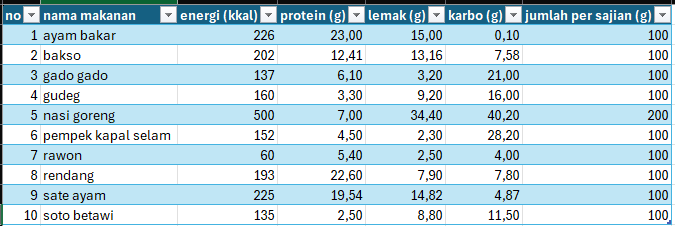
\includegraphics[width=0.9\textwidth, center]{images/data-nutrisi.png}
    \caption{Hasil pengumpulan data nutrisi makanan dari situs nilaigizi.com}
    \label{fig:data-nutrisi}
\end{afigure}

Proses pencarian data nutrisi makanan diimplementasikan ke dalam bentuk kode seperti yang dapat dilihat pada blok program di bawah:

\begin{lstlisting}[style=customc]
def predict_class_with_nutrition(model, images, 
show = True):
  for img in images:
    img = image.load_img(img, target_size=(224, 224))
    img = image.img_to_array(img)
    img = np.expand_dims(img, axis=0)
    img = preprocess_input(img)

    preds = model.predict(img)
    class_labels = class_names
    pred = np.argmax(preds, axis=-1)
    predicted_class = class_names[pred[0]]
    predicted_prob = preds[0][pred[0]] * 100

    nutrition = data[data['nama makanan'].str.contains(
    predicted_class, case=False)]
    nutrition = nutrition.iloc[:, 1:]
    print("-" * 30)
    for col in nutrition.columns:
      print(f"{col.capitalize():>20}: 
      {nutrition[col].iloc[0]:}")
    print("-" * 30)

    if show:
        plt.imshow(img[0].astype('uint8'))
        plt.axis('off')
        plt.title(f"{predicted_class} 
        ({predicted_prob:.2f}%)")
        plt.show()
\end{lstlisting}








